\chapter{Usability Testing}
When we started this project the main reason was to simplify the administration systems to one single interface. So that there is only one code base and only one interface for the user to learn.\\
The first part should be given by default because we use a specialized system to run PHP code on the tablet. The system is called PAW \citep{paw} and is still in its beta phase.\\
The second part is the tricky part. There is only one interface to use, but it must be easy to learn and use so that the system does not have to be reworked.\\
That is why we have performed a usability test.\\
\\

%How did we do the test
	%Who was where
	%The simularity of the questions
The test was performed in Cassiopeias usability lab, where we had logged the computer onto our website. The setup of the usability lab is as displayed on figure \ref{fig:usabilitylab}. We did not use the second room.\\
Each test person was lead into the test room, offered a cup of coffee and then we started the prepared briefing, everyone was given the same briefing and we asked them to sign a consent form that they were being tapped for research purposes.\\
After this we asked them to execute a set of assignments within the system, always the same assignments, designed to lead them around the whole active system. \fix{Add a refference to appendix with questions and briefing}\\
We had the same one person sit in the room to assist the user, both to give them their assignment and to tell them when they had completed it. All assignments was kept very short, as to not disturb the user more then needed.\\
When the user had completed all the assignments we had the two men that sat in the control room come and help ask questions to the test person about some of the ways the test person used the system.\\
\\

\begin{figure}[htbp]
	\centering
		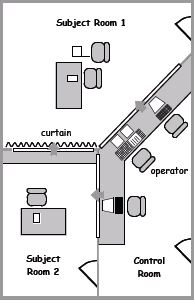
\includegraphics[width=0.80\textwidth]{images/usabilitylab.png}
	\caption{Usability Lab}
	\label{fig:usabilitylab}
\end{figure}

	%Picking the candidates
This test was only performed on 4 persons, this might not sound as many. But being that there is only a few persons in Denmark that will use the administration features that we have designed. We had to make an expert test, and use the gathered data as such. We only had one person available that we thought would use the main system that we have designed, but this person who is responsibly for a kinder garden, is not even high enough up in their system to be using most of the admin features. But this is all we had to go on, as we had no way of contacting the persons who is in a high enough position to be the intended user.\\
So the test was carried out with the one person to be the actual test person, and the 3 others be confirmation test, so that we did not draw conclusions from one test, that could be a result of lacking computer skills or other variables of the same sort.
	
	%The old version
	
%Result of the test
\begin{table}[htbp]
	\centering
		\begin{tabular}{|l|l|l|l|}
			\hline
			Name & Type & Severity & Done\\\hline
			Create Picto Categories & It is not possible to create new categories of Pictos & Critical &\\\hline
			Profile Picture View & The accept button hard to find at the end of a page with scroll & Serious &\\\hline
			Language at Profile Picture & The word change as accept button was misleading & Serious &\\\hline
			Profile Picture Placeholder & The GIRAF Logo as Placeholder is misleading  & Cosmetic & Done\\\hline
			Language Support on Index site & Did not change to danish & Critical &\\\hline
			Profile Picture �Edit� Button & Edit is not fully narrative & Cosmetic &\\\hline
			Edit Department in Own Profile Site & The department should be a link and not editable & Serious & (Done)\\\hline
			Missing Links in Own Profile & Links from Own Profile's relations is missing & Serious & \\\hline
			Loading Time of Own Profile Site & Getting Own Profile site takes too long time & Cosmetic &  \\\hline
			QR Edit Opportunities & Restrict editing QR only to department manager & Critical &  \\\hline 
			Language Understanding in Menu & �Add� and �Make� under Pics Manager is not narrative & Serious & \\\hline
			Navigation in Menu & It is not rational to have �Add Relation� before �Create Profile� & Cosmetic & Done \\\hline
			Standardize Accept and Submit buttons & Too many variations of �Change�, �Submit�, �Save� & Cosmetic & \\\hline
	\end{tabular}
	\caption{Bugs/Errors Found Under Usability Testing}
	\label{tab:Bugs/Errors}
\end{table}

-	Link errors on own profile �child�? %Hvilken fejl?
-	Something is wrong with rights for editing pictograms according to responsibility persons. (Det skal v�re muligt for alle pedagoger I en afdeling at redigere og tilf�je pictogrammer til alle b�rn i afdelingen) %Skal de det kunne det.
-	Admin functions is supposed to be used by someone higher up than our contact person, who is the administrator of a department.
	%Bugs/Errors
		%Severity
	%Features
\begin{table}[htbp]
	\centering
		\begin{tabular}{|l|l|l|}
			\hline
			Name & Type & Done\\\hline
			Linkes in Profiles Site & The linkes to profiles in Profiles site &\\\hline
			Customize Modal & Make the modal to take more input for a more Customize modal  &\\\hline
			Form Feature & Make is possible to push enter to save in form &\\\hline
			Recording Feature & Record sound in browser to Picto Create&\\\hline
			Standardize Input Text & All input text in form is transformed to Starting letter uppercase and rest lowercase &\\\hline  
			Better Navigation in Profiles & Add �add relations� and �create profile� navigation in Profiles & \\\hline  
		\end{tabular}
	\caption{Features Found Under Usability Testing}
	\label{tab:NewFeature}
\end{table}	
	-	Auto add �inline-text� to image preview (Pictogram feature)%Forst�r jeg ikke lige
	-	Create Pictogram from kids profile
%What have we already fixed

%What MUST be fixed

%What could be added later - Maybe a refference to Future Work instead?